\documentclass[a4paper,12pt]{article}

\usepackage{cmap}		
\usepackage[utf8]{inputenc}			
\usepackage[english, russian]{babel}
\usepackage{framed}
\usepackage{hyperref}
\usepackage{amsmath}
\usepackage{graphicx}
\usepackage{wrapfig}
\usepackage{lipsum}
\usepackage{listings}
\usepackage{color}
\usepackage{indentfirst}
\usepackage{times}
\usepackage{textcomp}
\usepackage{changepage}
\makeatletter
\newenvironment{restoretext}%
    {\@parboxrestore%
     \begin{adjustwidth}{}{\leftmargin}%
    }{\end{adjustwidth}}
\makeatother

\addto\captionsrussian{\def\refname{Список литературы}}
\newcommand{\HRule}{\rule{\linewidth}{0.5mm}}

\begin{document}

\begin{titlepage}
\begin{center}


\includegraphics[width=0.7\textwidth]{pics/logo.png}

\textsc{\normalsize Московский Государственный Университет имени М. В. Ломоносова}\\
\textsc{\small Факультет Вычислительной Математики и Кибернетики}\\
\textsc{\small Кафедра Системного Программирования}\\[1.5cm]

\textsc{\Large Курсовая работа }\\[0.5cm]
\textsc{ \bf \Large  Извлечение логической структуры из сканированных документов }\\[1.2cm]

\vspace{3cm}
\begin{flushright}
Автор: \\
группа 328 \\
Богатенкова Анастасия Олеговна
\end{flushright}
\begin{flushright}
Научный руководитель: \\
Козлов Илья Сергеевич
\end{flushright}

\vspace{3cm}
{ Москва, 2020}\\[0.2cm]

\vfill

\end{center}
\end{titlepage}

\tableofcontents

\newpage 
\section*{Введение}\addcontentsline{toc}{section}{Введение}

Большое количество текстовой информации представлено в виде pdf-документов, причем эти документы могут быть сканированными копиями бумажных носителей и у них может отсутствовать текстовый слой. При этом размер документов может быть очень большим. Зачастую требуется осуществлять поиск по содержимому таких документов и желательно осуществлять это более эффективным способом.

Как правило, документы имеют логическую структуру и содержат название, разбиение на главы, подглавы и т. д., нумерованные и маркированные списки. Выделение такой логической структуры документа может помочь при решении задач автоматизированного анализа документов, а также при поиске по документам.

Применяется множество разнообразных подходов, которые позволяют выделять в тексте заголовки и распознавать логическую структуру документов.
Для эффективного извлечения такой структуры может быть необходима метаинформация, такая как размер и тип шрифта, отступы, междустрочные интервалы и т. д. 
Поэтому извлечение логической структуры логично делать на этапе анализа сканированных документов.

\newpage
\section{Постановка задачи}

Целью моей курсовой работы является разработка метода выделения логической структуры из документов. Рассмотрим структуру документа в виде глав, подглав (и т. д.), элементов нумерованных и маркированных списков.
Поставим задачу следующим образом: необходимо классифицировать каждую строчку документа как заголовок, элемент списка или текст.

При решении задачи можно выделить следующие этапы ее выполнения:

\begin{enumerate}
\item Описание конкретной логической структуры, которую нужно выделить, т. е. разработка манифеста.

\item Разметка корпуса документов для обучения классификатора. Разметка проводится по правилам, указанным в манифесте. 

\item Реализация метода и проведение экспериментальной проверки разработанного метода.
\end{enumerate}

Ограничим класс документов, с которыми будем работать, сканированными документами без текстового слоя. Будем считать, что в документах не содержатся изображения и таблицы. 

\newpage
\section{Обзор существующих решений}

По извлечению структуры из документов существуют несколько подходов:
\begin{itemize}
\item на основе оглавления;
\item на основе правил;
\item на основе машинного обучения.
\end{itemize}

\subsection{Извлечение структуры из документов на основе оглавления и правил}

По анализу документов проводится очень много соревнований на ICDAR, например \cite{link1,link2,link3}. В одном из таких соревнований \cite{link1} производилось извлечение структуры из книг, содержимое которых было получено с помощью оптического распознавания символов. Структура книг в виде разбиения на страницы, параграфы, главы извлекалась с использованием оглавления, которое присутствовало в большинстве книг. 

В 2019 году проводились соревнования FinTOC \cite{link4}, где из финансовых документов извлекалась структура в виде иерархии уровней заголовков документов. Максимальная глубина уровней равна пяти. Одна из команд-участниц \cite{link5} извлекала необходимую структуру используя оглавление документов, а также систему правил, которые применялись для определения иерархии заголовков.
Сначала идентифицировались страницы, содержащие текст оглавления, затем в документе находились страницы, соответствующие заголовкам, указанным в оглавлении. 
Последним шагом являлось выделение иерархии найденных заголовков, основанное на применении правил: анализировались такие признаки, как междустрочный интервал, отступ, шрифт, символы нумерации.
Использованный подход позволил получить достаточно высокую точность, но низкую полноту, так как некоторые оглавления документов были неполными.

Извлечение структуры документов на основе оглавления имеет ряд недостатков. Во-первых, невозможно обрабатывать документы, в которых нет оглавления. Во-вторых, при использовании этого метода в структуру документа не будут включаться заголовки, которые не вошли в оглавление, например заголовки более низкого уровня. В-третьих, для нашей задачи необходимо извлекать элементы маркированных и нумерованных списков, которые не включаются в оглавление документа.

\subsection{Извлечение структуры из документов на основе машинного обучения}

В соревнованиях \cite{link4} кроме извлечения иерархической структуры документов решалась задача определения, является ли конкретный блок документа заголовком. Командам был дан набор pdf-документов, xml-файлов с выделенными блоками документов, а так же набор признаков для каждого блока: является ли шрифт блока жирным, курсивом, состоит ли текст из заглавных букв, начинается с заглавной буквы или с нумерации. Кроме данных признаков, каждая из команд использовала различные дополнительные морфологические, семантические, лингвистические признаки. На основе этих признаков обучались различные классификаторы: SVM, MNB, Extra Tree, Decision Tree, Gradient Boosting. Для оценки результатов использовалась F1-мера, максимальный score в соревновании -- 0,982.

Победители соревнования \cite{link6} создали новый датасет для обучения с помощью аугментации данных, перевели новые сгенерированные текстовые блоки в векторное представление, а затем использовали рекуррентные нейронные сети LSTM и BiLSTM для решения задачи классификации. Процесс аугментации показан на схеме ниже.

\begin{center}
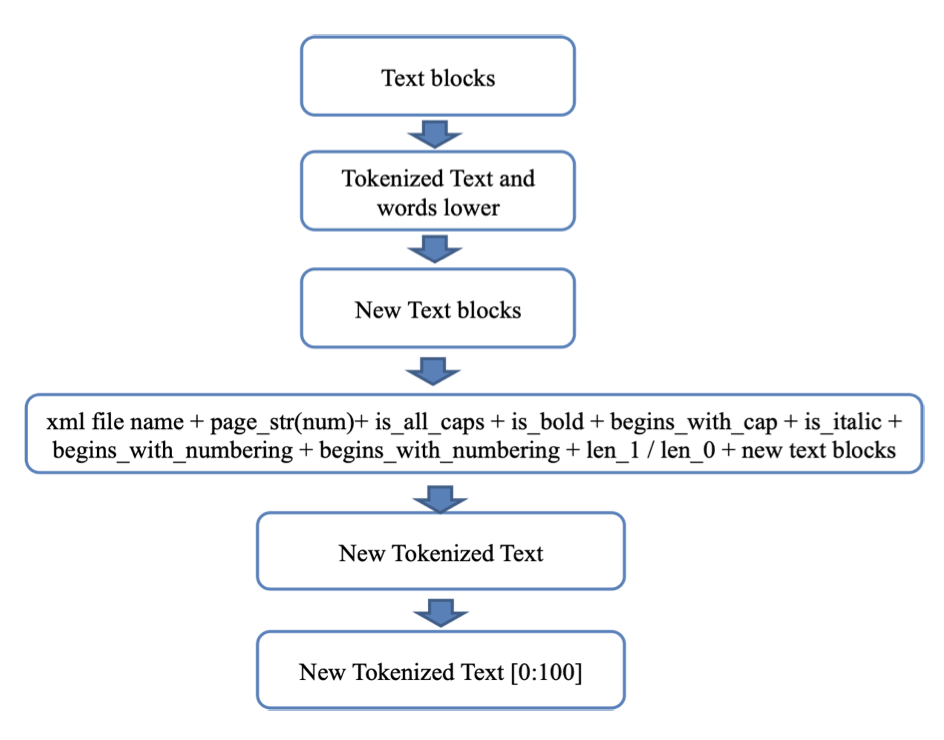
\includegraphics[height=0.5\textwidth]{pics/augmentation.png}
\end{center}

В статье \cite{link7} 2017 года структура документа извлекалась с использованием методов машинного обучения, включая глубокое обучение. Цель данной работы -- автоматически идентифицировать и классифицировать различные секции документов и понять их смысл в рамках документа (назначить семантическую метку). В рамках моей задачи интересна классификация секций документа.

\begin{center}
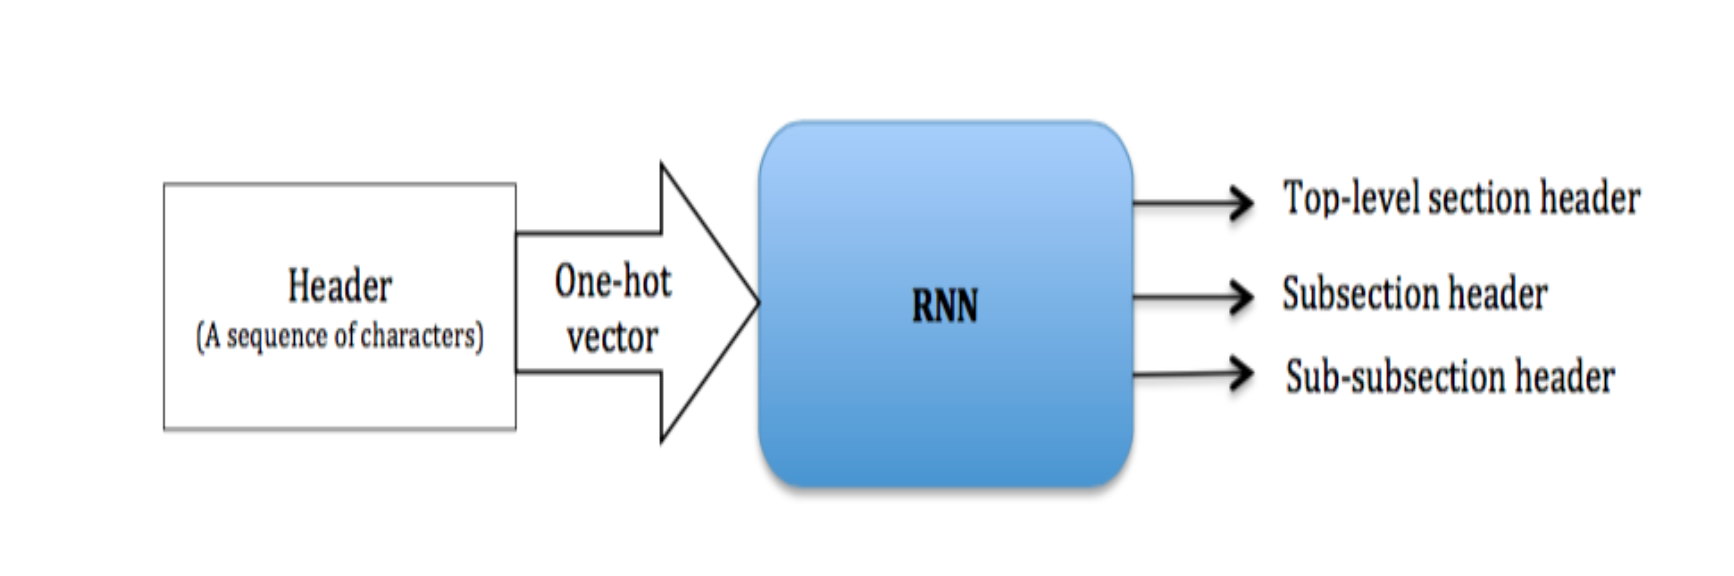
\includegraphics[width=1.0\textwidth]{pics/classifier.png}
\end{center}

Классификатор, который был использован при решении задачи, состоит из нескольких частей. Сначала строки документа подаются на вход классификатору (классификатор строк), который определяет, является ли строка заголовоком, затем строки-заголовки классифицируются точнее другими классификаторами (классификаторы секций). В этом решении структура документа имела вложенность 3, то есть предполагалось выделение секций, подсекций, подподсекций.
Кроме того, в данной работе был размечен датасет, на котором происходило обучение модели. Метрика качества - F1-мера, при идентификации заголовков итоговый score -- 0,96; при классификации секций средний F1-score -- 0,81.

Существующие решения использовать сложно, так как, во-первых, документы, с которыми необходимо работать, могут содержать заголовки или элементы нумерованных списков глубокой вложенности, например 1.1.1.1 (уровней вложенности может быть и больше), а внутри этих уровней могут располагаться нумерованные/маркированные списки, также вложенные.

Во-вторых, как правило в существующих решениях основное внимание уделялось выделению структуры в виде заголовков, для нашей задачи требуется также определять элементы списков.

В-третьих, в большинстве примеров, приведенных выше, осуществляется классификация текстовых блоков, в нашей задаче необходимо классифицировать каждую строку документа.

\newpage
\section{Описание практической части}

\subsection{Описание логической структуры}

Для того, чтобы классифицировать каждую строку документа, необходимо определить, по какому принципу конкретная строка будет относиться к тому или иному классу. Это необходимо при осуществлении разметки корпуса документов для обучения классификатора. 

С этой целью был разработан манифест, прикрепленный в приложении.

\subsection{Обоснование выбранного инструментария}

В качестве языка реализации был выбран Python, так как для данного языка программирования разработано множество необходимых при решении задачи библиотек, а именно:

\begin{itemize}
\item \href{https://opencv.org}{opencv} -- библиотека для работы с изображениями (библиотека компьютерного зрения и машинного обучения);
\item \href{https://pypi.org/project/pytesseract/}{pytesseract} -- обертка над программой tesseract, предназначенной для распознавания текста на изображении;
\item \href{https://scikit-learn.org}{sklearn} -- библиотека для решения различных задач машинного обучения.
\end{itemize}

\subsection{Подготовка датасета для обучения}

Для обучения классификатора строк необходимо иметь размеченный корпус документов. Для этой цели был использован набор документов в виде изображений в формате .jpeg, скачанный из интернета. Документы содержат тексты договоров различных предприятий (СТО, РД ЭО и др.). 

Документы были размечены с использованием системы для разметки, разработанной в ИСП РАН \cite{link8}. Данная система разметки с помощью библиотеки pytesseract позволила выделить в документах без текстового слоя строки текста, а также рамки, заключающие в себе эти текстовые строки (bounding boxes). То есть результатом разметки стал набор .json файлов, каждый из которых содержал название документа и список текстовых строк с координатами заключающих их рамок и правильными метками.

Для проверки логичности манифеста и правильности разметки была посчитана специальная статистика \href{https://en.wikipedia.org/wiki/Cohen%27s_kappa}{Cohen's kappa}. Данная статистика позволяет оценить меру согласия между аннотаторами при решении задачи классификации. Коэффициент согласованности можно посчитать следующим образом:

$$ \kappa \equiv {\frac {p_o-p_e}{1-p_e}}=1-{\frac {1-p_o}{1-p_e}},$$
где $p_o$ - вероятность согласованности меток, приписанных аннотаторами (точность), $p_e$ - вероятность того, что согласие аннотаторов достигнуто в результате случайной разметки.

После разметки десяти документов значение статистики $\kappa$ оказалось равным 0.975, после чего было решено размечать остальной корпус документов. В результате было размечено 600 документов и отдельные .json файлы были объединены в один, использующийся для обучения классификатора.

\subsection{Выделение признаков}

Для каждой размеченной строки документа необходимо определить набор характеризующих её числовых признаков, которые нужно выделить. Далее выделенный вектор признаков подается на вход классификатору.

Среди всех признаков можно выделить следующие группы:

\begin{itemize}

	\item Признаки, основанные на регулярных выражениях.

	Данная группа признаков основывается на анализе начала и конца каждой строки. Такие признаки очень важны для выявления элементов списков различных типов, а также могут сигнализировать о конце заголовка или начале списка.

	Например, для каждой строки анализировалось следующее:

	\begin{itemize}

		\item[--] с помощью регулярных выражений специального вида выявлялось, начинается ли строка с цифры или буквы со скобкой или точкой (также анализируются иерархические выражения вида 1.1.1);
		\item[--] начинается ли строка с тире (и других символов, характерных для маркированного списка);
		\item[--] состоит ли строка целиком из заглавных букв (характерно для некоторых заголовков);
		\item[--] начинается ли строка с заглавной (строчной) буквы;
		\item[--] начинается ли строка с конкретных слов типа «Раздел», «Секция», «Глава» и т. д.;
		\item[--] оканчивается ли строка символами вида «. , ; :»;
		\item[--] оканчивается ли строка строчной буквой.

	\end{itemize}

	\item Текстовые признаки.

	Данная группа признаков связана с подсчетом некоторых строковых характеристик, а именно:

	\begin{itemize}

		\item[--] количество букв в первом и втором словах строки;
		\item[--] количество слов в строке (строка разбивается на слова по пробелам);
		\item[--] количество символов в строке (длина строки).

	\end{itemize}

	\item Визуальные признаки.

	Данная группа признаков связана с графическим представлением текста в документе. То есть при анализе строки рассматривается не ее текст, а следующие признаки:

	\begin{itemize}

		\item[--] отступ от левого края страницы;
		\item[--] высота текста строки (точнее высота ограничивающей ее рамки);
		\item[--] отступ от верхнего края страницы;
		\item[--] с помощью специальных функций определялась жирность шрифта различных уровней. 

	\end{itemize}

\end{itemize}

Кроме того, к признакам, перечисленным выше, для каждой строки были добавлены аналогичные признаки четырех предыдущих и следующих строк. Это полезно для анализа продолжения блока строк конкретного типа.

Для строк, которые начинаются с нумерации, определялось, есть ли в документе строка, предшествующая данной с нумерацией, меньшей данной на единицу.

И, наконец, для каждого документа вычислялся средний отступ от левого края страницы, средняя высота шрифта, средняя длина строки, среднее число слов в строках, среднее значение дли жирности шрифта, среднее число букв в первом слове каждой строки. Данные значения добавлялись к признакам каждой строки документа.

\subsection{Подбор классификатора}

При решении задачи было опробовано множество классификаторов, для лучших из них проведен анализ результатов. В анализе участвовало 4 классификатора:

\begin{itemize}

	\item алгоритм k ближайших соседей (\href{https://scikit-learn.org/stable/modules/generated/sklearn.neighbors.KNeighborsClassifier.html}{KNeighborsClassifier});
	\item логистическая регрессия (\href{https://scikit-learn.org/stable/modules/generated/sklearn.linear_model.LogisticRegression.html}{LogisticRegression});
	\item градиентный бустинг (\href{https://scikit-learn.org/stable/modules/generated/sklearn.ensemble.GradientBoostingClassifier.html}{GradientBoostingClassifier});
	\item экстра-градиентный бустинг (\href{https://xgboost.readthedocs.io/en/latest/}{XGBClassifier}).

\end{itemize}

Множество документов тремя способами было разбито на тренировочное и тестовое множества (разбиение по документам), на каждом разбиении было проведено обучение классификаторов и вычисление F1-score. Усредненные значения F1-score для каждого классификатора показаны на графике ниже:

\begin{center}
	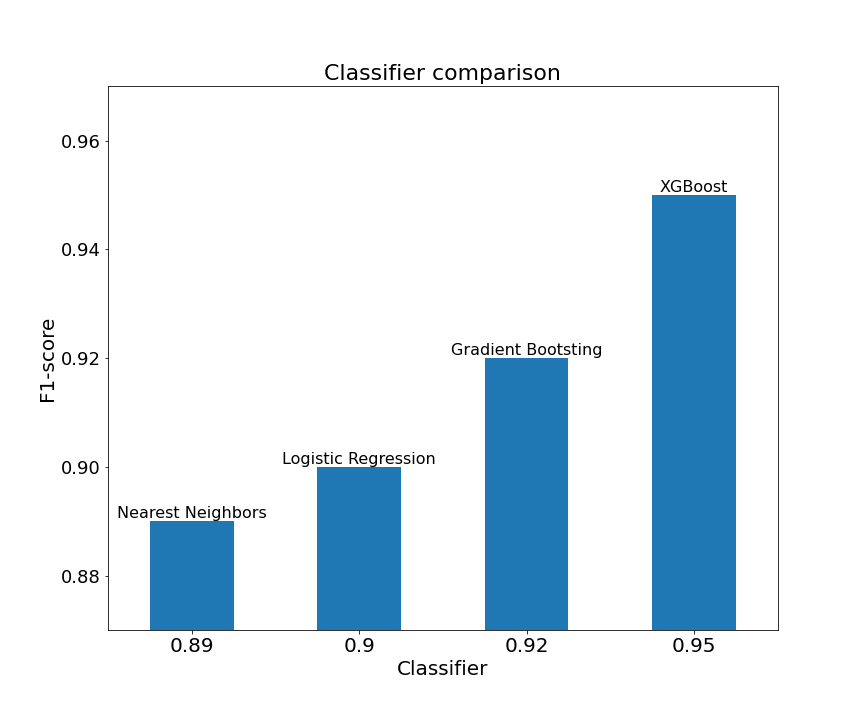
\includegraphics[width=1.0\textwidth]{pics/scores.png}
\end{center}

На графиках, изображенных ниже, точками показано распределение множеств строк документов различных типов по двум признакам: горизонтальная ось соответствует величине отступа строки от левого края страницы, вертикальная ось соответствует значению жирности шрифта. При этом красному цвету соответствуют строки-заголовки, зелёному -- списки, синему -- текст, желтому -- всё остальное. В первом столбце изображено правильное распределение строк, остальные столбцы соответствуют результатам предсказаний классификаторов.

\begin{center}
	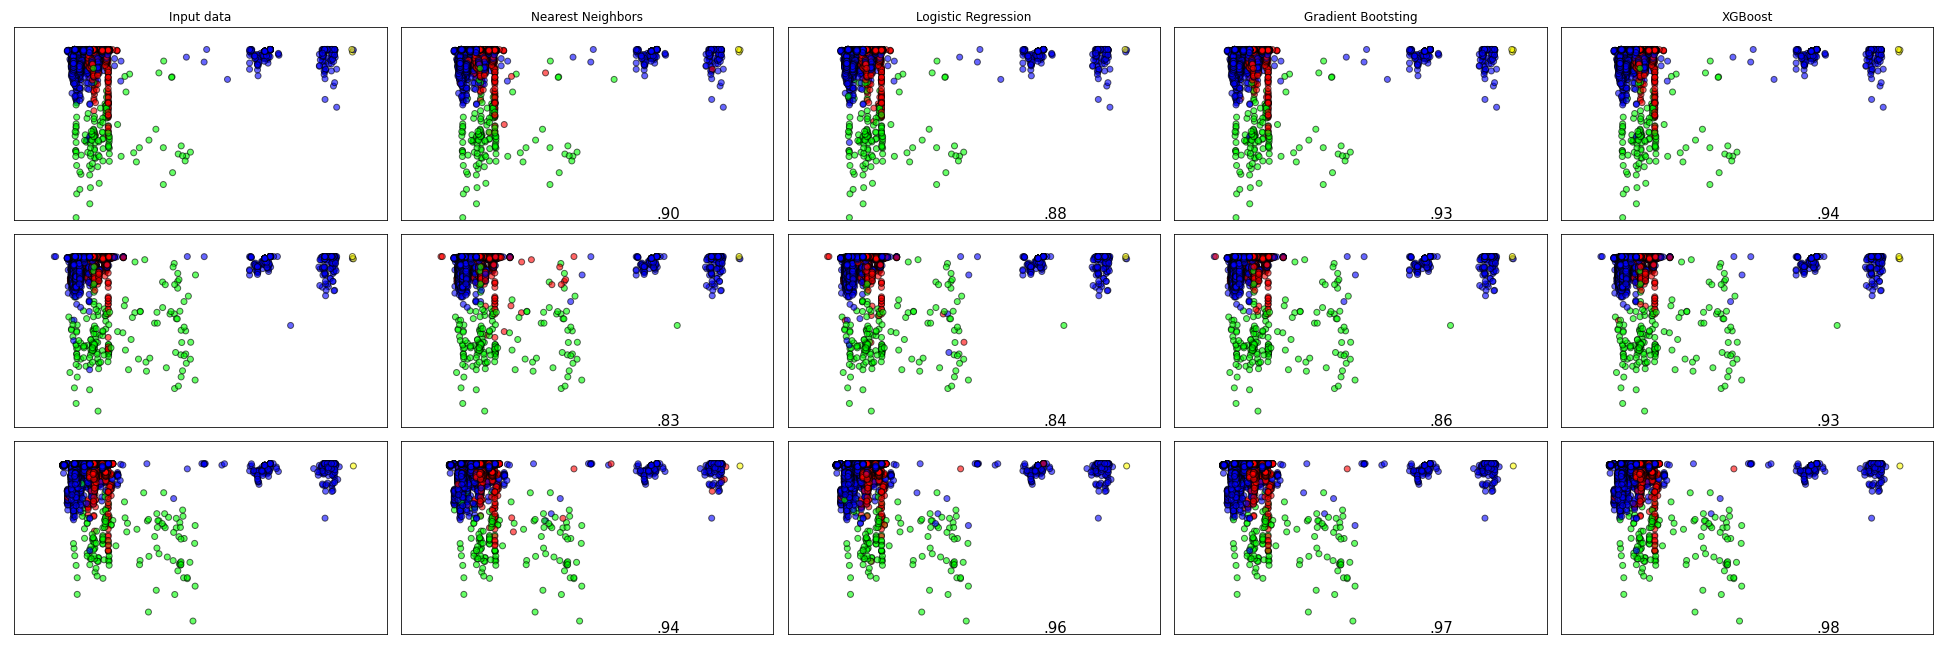
\includegraphics[width=1.0\textwidth]{pics/graphics.png}
\end{center}

Судя по графикам, по данным двум признакам достаточно легко спутать текст и список по величине отступа, а заголовок и текст по жирности шрифта (однако на графиках не учитываются другие признаки).

Отдельные группы точек справа соответствуют строкам с номерами страниц документов. Как правило, нумерация страниц располагается внизу по центру или в правом нижнем углу страницы. Некоторые классификаторы относят такие строки к типу «Другое».

В целом, все рассмотренные классификаторы показали хороший результат, наилучший результат показал XGBClassifier, поэтому было решено выбрать его.

\subsection{Анализ важности признаков}

Анализ значимости признаков был проведен с помощью библиотеки \href{https://github.com/limexp/xgbfir}{xgbfir}.
Ниже представлены первые 10 признаков с наивысшей важностью. Это признаки, которые имеют наибольший вес при вычислении предсказания классификатора.

\begin{center}
	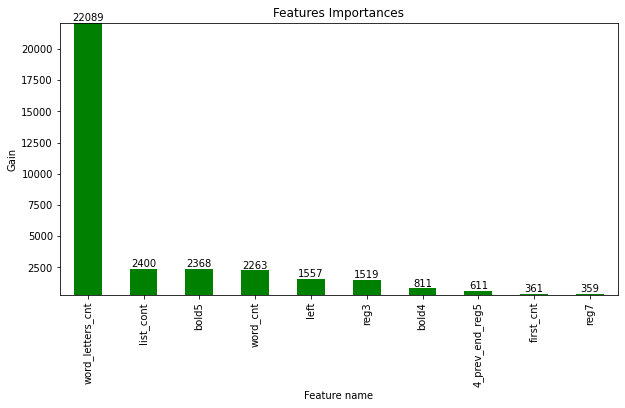
\includegraphics[width=1.0\textwidth]{pics/gaines.png}
\end{center}

Описание признаков:

\begin{itemize}

	\item $word\_letters\_cnt$ -- число символов первого слова в строке (слова разделяются пробелами);
	\item $list\_cont$ -- признак для строк, являющихся элементами списка, принимающий значение булевого типа: True, если перед данной строкой в документе найдена строка, являющаяся предыдущим элементом данного списка и False иначе;
	\item $bold5$ -- признак жирности шрифта (число 5 означает размер ядра свертки для определения уровня жирности);
	\item $word\_cnt$ -- число слов в строке;
	\item $left$ -- отступ от левого края страницы;
	\item $reg3$ -- признак начала строки с выражения вида 1.1.1 (произвольный уровень вложенности, вместо цифр могут быть буквы);
	\item $bold4$ -- признак жирности шрифта с размером ядра свертки, равным 4;
	\item $4\_prev\_end\_reg5$ -- признак, заканчивается ли предыдущая строка буквой;
	\item $first\_cnt$ -- число букв в начале строки;
	\item $reg7$ -- признак начала строки с тире.

\end{itemize}

С использованием данных о важности признаков, в признаковое пространство были добавлены новые признаки. Например, вместо одного признака, отвечающего за жирность шрифта, была добавлена целая группа признаков, отвечающая за различные уровни жирности шрифта. Для самых важных признаков к вектору признаков каждой строки документа были добавлены усреднённые значения данных признаков по документу.

На графике выше представлен итоговый список признаков и значения их важности.

\subsection{Настройка параметров XGBClassifier}

Градиентный бустинг — это алгоритм машинного обучения, который строит модель предсказания в форме ансамбля слабых предсказывающих моделей (например, деревьев решений).

В нашем случае, при использовании XGBClassifier, для настройки доступны три группы параметров:

\begin{itemize}

	\item параметры, отвечающие за общее функционирование алгоритма (тип предсказывающей модели, число нитей для запуска);
	\item параметры для предсказывающей модели, в нашем случае это дерево (шаг обучения, максимальная глубина, параметры регуляризации и т. д.);
	\item параметры, задающие функцию потерь для минимизации и метрику для оценки качества.

\end{itemize}

Мы сосредоточимся на подборе параметров второй группы.

Настройка параметров классификатора проводилась по алгоритму, предложенному в \cite{link9}:

\begin{enumerate}

	\item выбирается относительно высокий шаг обучения ($learning\_rate$), для которого подбирается количество деревьев ($n\_estimators$);
	\item подбираются параметры деревьев ($max\_depth, min\_child\_weight,$ $gamma, subsample, colsample\_bytree$) для выбранного шага и количества деревьев;
	\item настраиваются параметры регуляризации ($lambda, alpha$) для снижения сложности модели и улучшения производительности; 
	\item понижается шаг обучения и выявляются оптимальные параметры.

\end{enumerate}	

На графике ниже представлено изменение F1-score в процессе подбора параметров. 

\begin{center}
	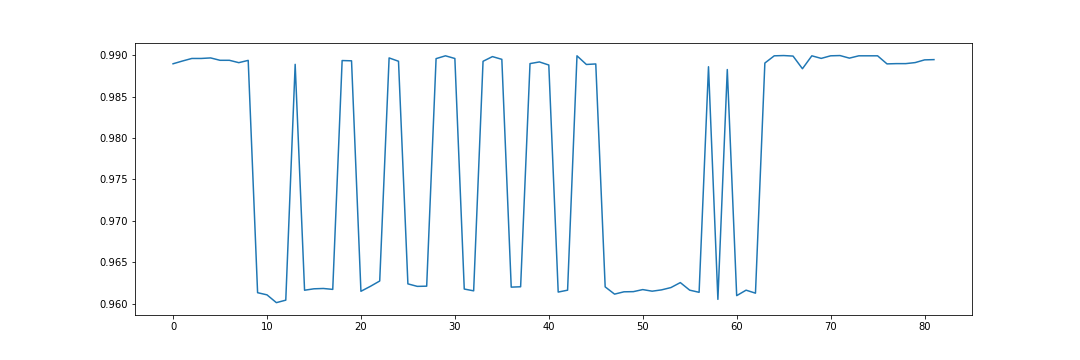
\includegraphics[width=1.0\textwidth]{pics/parameters.png}
\end{center}

Параметры итоговой модели:

$learning\_rate = 0.1$

$n\_estimators = 1000$

$max\_depth = 7$

$min\_child\_weight = 2$

$gamma = 0$

$subsample = 1$

$colsample\_bytree = 1$

$alpha = 0.01$

Итоговый F1-score, полученный в результате кросс-валидации:

 $0.98995$

 \subsection{Анализ ошибок классификатора}

 На графике ниже показана \href{https://en.wikipedia.org/wiki/Confusion_matrix}{матрица ошибок} для полученного классификатора. По вертикальной оси расположены правильные классы, по горизонтальной - классы, которые предсказал классификатор. В клетках на пересечении расположены значения количества строк, у которых совпали данные классы.

\begin{center}
	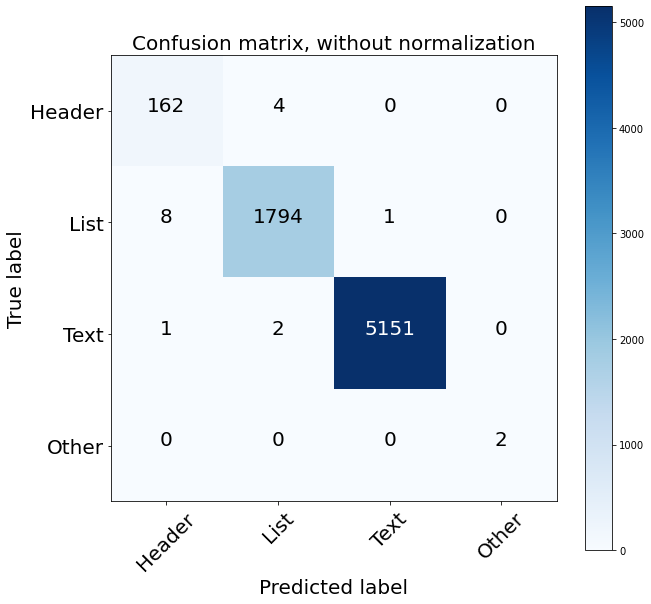
\includegraphics[width=1.0\textwidth]{pics/conf_matrix.png}
\end{center}

На графике видно, что 8 строк, относящихся к типу «Список», были проклассифицированы как «Заголовок», 4 строки, напротив, вместо метки «Заголовок» получили метку «Список». Аналогичную статистику можно посмотреть и для других пар классов.

Таким образом, больше всего классификатор путает классы «Заголовок» и «Список». Это можно объяснить тем, что некоторые признаки данных классов очень похожи, например, многие заголовки начинаются с нумерации, а элементы списков имеют большой отступ от левого края страницы.

\newpage
\section*{Заключение}\addcontentsline{toc}{section}{Заключение}

В рамках моей курсовой работы был реализован алгоритм классификации строк документа, определяющий в документах заголовки и списки разных уровней вложенности.

\begin{itemize}

\item Разработан манифест, описывающий каждый из типов строк, размечен копус документов, используемый в качестве тренировочных данных.

\item Выявлены признаки, наиболее подходящие для обучения классификатора, проанализирована их важность. 

\item Выбран наиболее подходящий классификатор, для которого были подобраны оптимальные параметры.

\item Проведен анализ, на каких строках классификатор ошибается чаще всего.

\end{itemize}

Дальнейшие исследования могут быть направлены на определение уровней вложенности строк различных типов.

\newpage
 
\addcontentsline{toc}{section}{Список литературы}
 \begin{thebibliography}{}
    \bibitem{link1} \href{https://hal.archives-ouvertes.fr/hal-01073396/document}{Antoine Doucet, Gabriella Kazai, Sebastian Colutto, Günter Mühlberger. Icdar 2013 competition on book structure extraction. 12th International Conference on Document Analysis and Recognition (ICDAR), 2013}
    \bibitem{link2} \href{https://ieeexplore.ieee.org/abstract/document/8270162}{Liangcai Gao, Xiaohan Yi, Zhuoren Jiang, Leipeng Hao, Zhi Tang. ICDAR2017 competition on page object detection. 14th International Conference on Document Analysis and Recognition (ICDAR), 2017}
    \bibitem{link3} \href{https://usir.salford.ac.uk/id/eprint/44369/1/ICDAR2017%20Competition%20on%20Recognition%20of%20Documents%20with%20Complex%20Layouts.pdf}{C. Clausner, A. Antonacopoulos, S. Pletschacher. ICDAR2017 competition on recognition of documents with complex layouts – RDCL2017. 14th International Conference on Document Analysis and Recognition (ICDAR), 2017}
    \bibitem{link4} \href{https://www.aclweb.org/anthology/W19-6407.pdf}{Rémi Juge, Najah-Imane Bentabet, Sira Ferradans. FinTOC-2019 Shared Task: Finding Title in Text Blocks.}
    \bibitem{link5} \href{https://www.aclweb.org/anthology/W19-6409.pdf}{Gael Lejeune Emmanuel Giguet. Daniel fintoc-2019 shared task: Toc extraction and title detection. In The Second Workshop on Financial Narrative Processing of NoDalida 2019, 2019}
    \bibitem{link6} \href{http://www.ep.liu.se/ecp/165/001/ecp19165001.pdf}{Ke Tian, Zi Jun Peng. Finance document extraction using data augmented and attention. In The Second Workshop on Financial Narrative Processing of NoDalida 2019, 2019.}
    \bibitem{link7} \href{https://dl.acm.org/doi/pdf/10.1145/3148055.3148080}{Muhammad Mahbubur Rahman, Tim Finin. Deep nderstanding of a Documents Structure. In 4th IEEE/ACM International Conference on Big Data Computing, Applications and Technologies, 2017}
    \bibitem{link8} \href{https://github.com/dronperminov/ParagraphLabelerApp}{ParagraphLabelerApp}
    \bibitem{link9} \href{https://www.analyticsvidhya.com/blog/2016/03/complete-guide-parameter-tuning-xgboost-with-codes-python/}{Complete Guide to Parameter Tuning in XGBoost with codes in Python}
\end{thebibliography}

\newpage
\section*{Приложение}\addcontentsline{toc}{section}{Приложение}

\textsc{\large Манифест}

\vspace{0.5cm}

Как правило, документы имеют логическую структуру: название, разбиение на главы, подглавы и т. д., нумерованные и маркированные списки. Мы занимаемся извлечением структурных элементов из сканированных документов. Выделение такой логической структуры документа может пригодиться для автоматизированного анализа документов. Мы хотим решать эту задачу как задачу классификации, нам нужно для каждой строки текста определить, к какому типу она относится.

Мы выделяем следующие типы строк: заголовок, элемент списка, текст.

На вход вам будут подаваться документы, в которых выделена прямоугольником одна строка. Вам необходимо для каждой выделенной строки документа определить её тип. Необходимо «Заголовок» пометить цифрой 1, «Список» - 2, «Текст» - 3, «Другое» - 4.

\begin{enumerate}

	\item Заголовок

	Название главы, секции, подглавы, параграфа. Строка помечается заголовком, если:

	\begin{itemize}
		\item текст визуально (полностью) выделяется жирностью;

		\vspace{0.5cm}

		\begin{restoretext}
		\frame{
\includegraphics[width=1.0\textwidth]{pics/1.png}}
		\end{restoretext}

		\item текст полностью выделяется шрифтом (курсив, подчеркнутый, другой шрифт, другой размер шрифта);

		\vspace{0.5cm}

		\begin{restoretext}
		\frame{
\includegraphics[width=1.0\textwidth]{pics/2.png}}
		\end{restoretext}

		при этом если текст строки выделен шрифтом частично, то заголовком это не считается;

		\vspace{0.5cm}

		\begin{restoretext}
		\frame{
\includegraphics[width=1.0\textwidth]{pics/3.png}}
		\end{restoretext}

		\item текст выделяется отступом (расположен по центру);

		\vspace{0.5cm}

		\begin{restoretext}
		\frame{
\includegraphics[width=1.0\textwidth]{pics/4.png}}
		\end{restoretext}

		\item если заголовок занимает несколько строк, остальные строки тоже относятся к типу «заголовок».

		\vspace{0.5cm}

		\begin{restoretext}
		\frame{
\includegraphics[width=1.0\textwidth]{pics/5.png}}
		\end{restoretext}

	\end{itemize}

	\item Список

	Начало нумерованного или маркированного списка. Строка помечается как элемент списка, если:

	\begin{itemize}
		\item строка наряду с несколькими другими строками пронумерована («1. 1) а) 1.1» и т. д. в начале строки);

		\vspace{0.5cm}

		\begin{restoretext}
		\frame{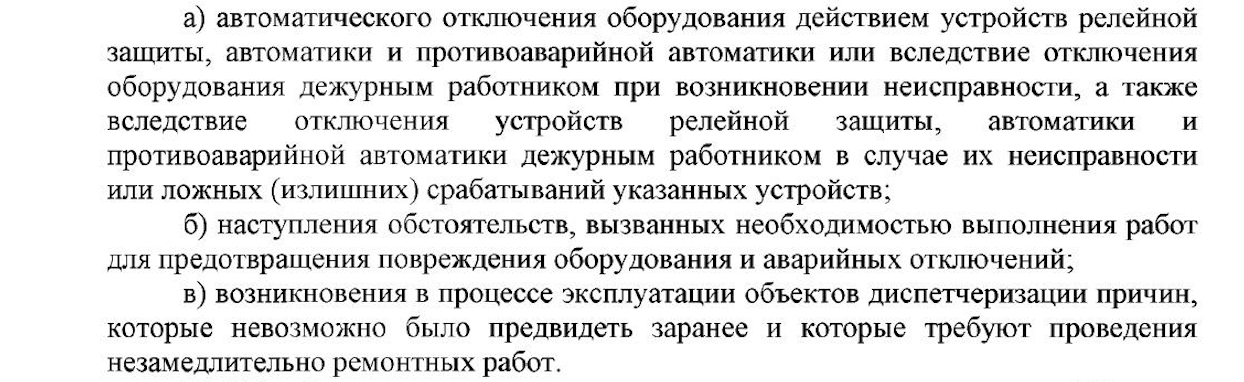
\includegraphics[width=1.0\textwidth]{pics/6.png}}
		\end{restoretext}

		\vspace{0.5cm}

		\begin{restoretext}
		\frame{
\includegraphics[width=1.0\textwidth]{pics/7.png}}
		\end{restoretext}

		\vspace{0.5cm}

		\begin{restoretext}
		\frame{
\includegraphics[width=1.0\textwidth]{pics/8.png}}
		\end{restoretext}

		На картинке выше как элемент списка будут помечены только две строки, остальные помечаются как текст.

		\item строка наряду с несколькими другими выделена некоторым маркером (точка, тире и т. д.) ;

		\vspace{0.5cm}

		\begin{restoretext}
		\frame{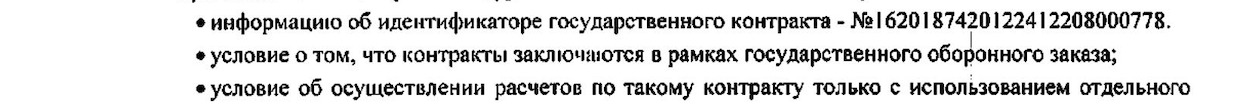
\includegraphics[width=1.0\textwidth]{pics/9.png}}
		\end{restoretext}

		\vspace{0.5cm}

		\begin{restoretext}
		\frame{
\includegraphics[width=1.0\textwidth]{pics/10.png}}
		\end{restoretext}

		В примере выше как элемент списка будут помечены только две строки, остальные помечаются как текст.

		\item если элемент списка визуально занимает несколько строк, все строки кроме первой помечаются как текст. Также к списку не относятся строки, помеченные как заголовок (выделенные шрифтом, жирностью и т. д.).

	\end{itemize}

	\item Текст

	Все остальные строки, содержащие текст документа, помечаются как текст.

\end{enumerate}

На вход вам будут подаваться документы, в которых выделена прямоугольником одна строка. Вам необходимо для каждой выделенной строки документа определить её тип. Необходимо «Заголовок» пометить цифрой 1, «Список» - 2, «Текст» - 3. В случае, если прямоугольником выделена строка, не содержащая текст (пустая строка, рукописная подпись, печать), строку необходимо пометить как «Другое» (цифра 4), либо пропустить данную строку при разметке.

Ниже приведен пример разметки. Красными прямоугольниками выделены заголовки, зелёными - элементы списков, а синими - текстовые блоки.

\begin{center}
\frame{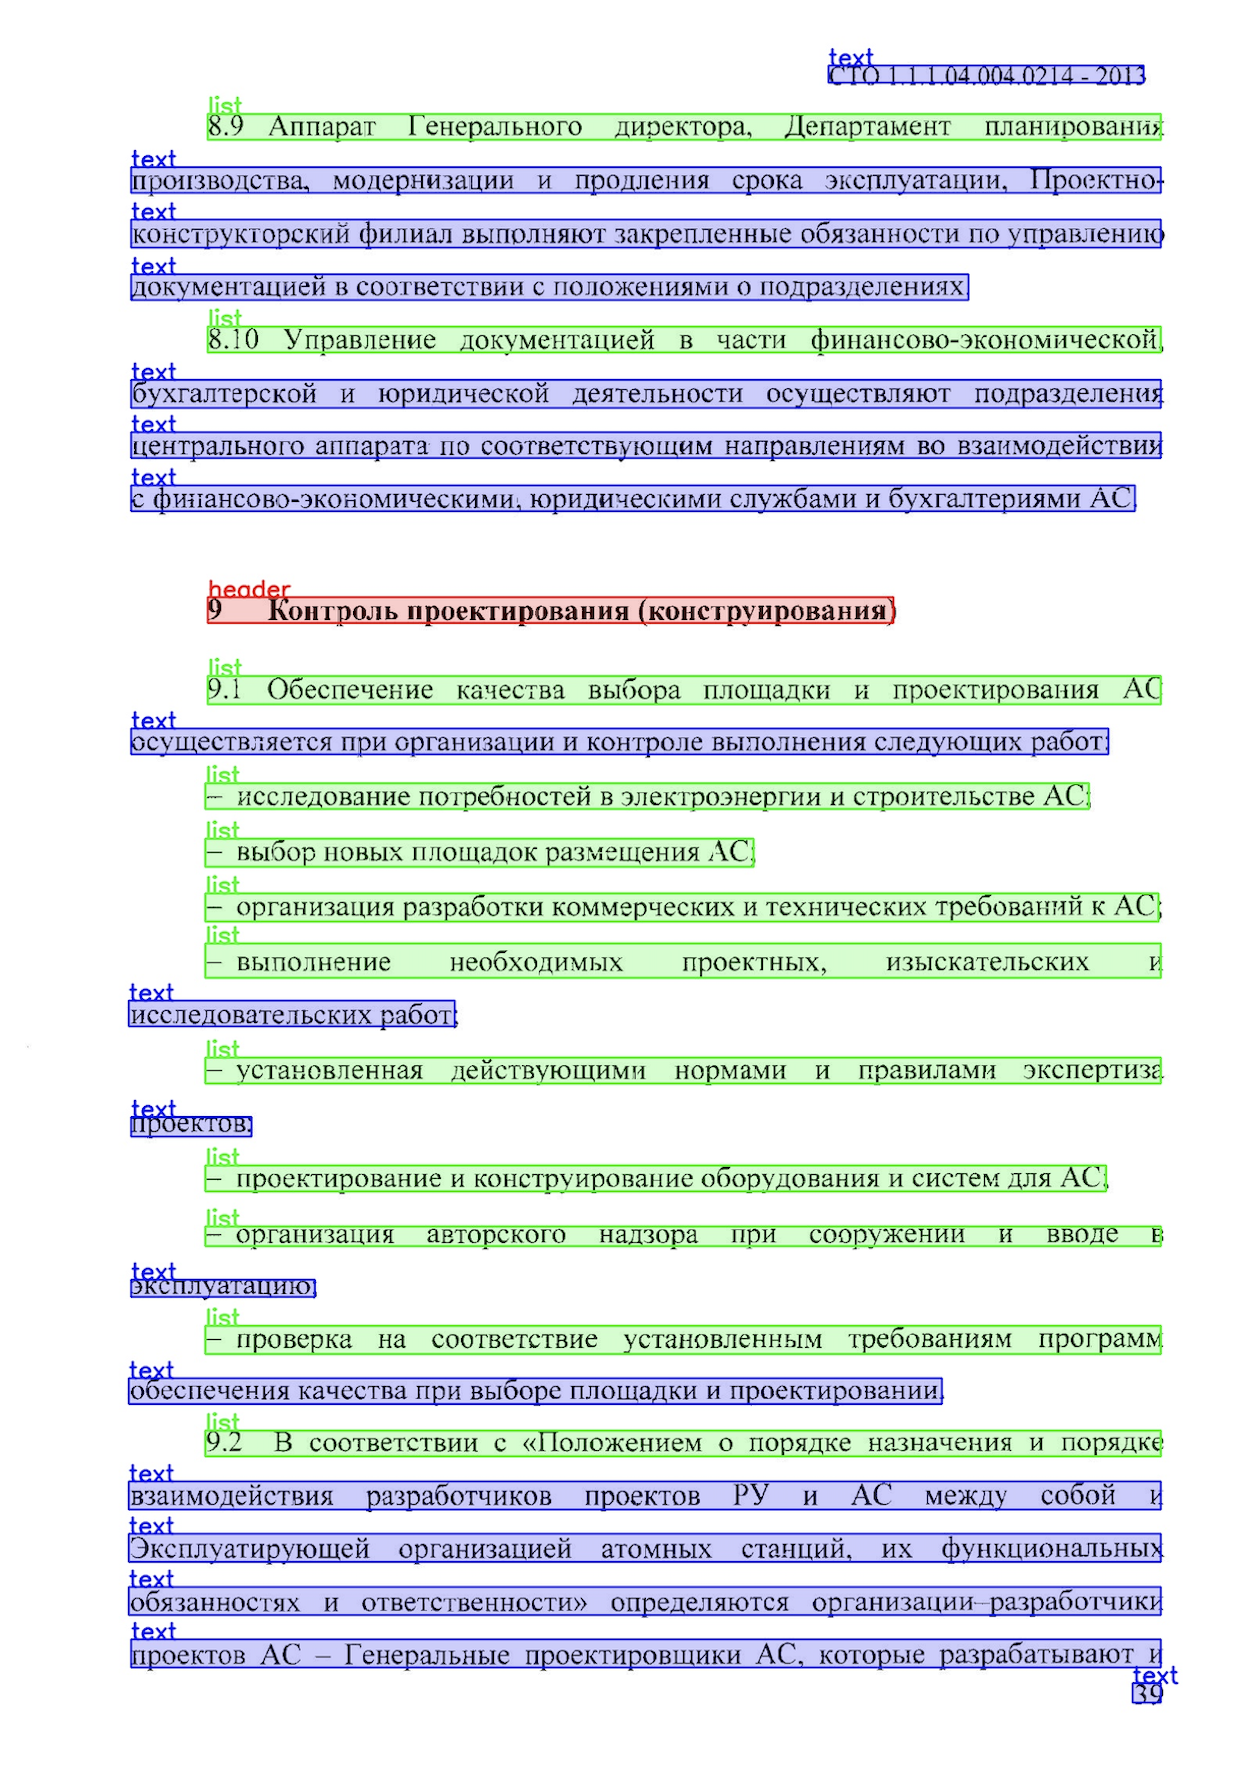
\includegraphics[width=1.0\textwidth]{pics/example.png}}
\end{center}

\end{document}
